\chapter{Affine toric varieties}

\section{Introduction}

\begin{definition}[Affine toric variety]
An \textbf{affine toric variety} is an irreducible affine variety $X$ equipped with an open embedding of a torus $T$ such that the translation action $T\times T\to T$ extends to an action of $T$ on $X$.
\end{definition}

\begin{remark}
The open torus is automatically dense in, and of the same dimension of, $X$.
\end{remark}

\begin{remark}
The extension of the action is unique because if $X$ and $Y$ are irreducible affine and $f,g:X\to Y$ agree on a dense open subset then $f=g$.
\end{remark}

\begin{example}
A torus is a toric variety.
\end{example}

\begin{example}
Affine space $\A^n$ is a toric variety, via the trivial embedding 
\[\G_m^n=\cpa{x_1\cdots x_n\neq 0}\subseteq \A^n.\]
\end{example}

\begin{example}
Let $C=V(x^3-y^2)\subseteq \A^2$ with torus
\[\funcDef{\G_m}{C}{t}{(t^2,t^3)}\]
and action
\[\funcDef{\G_m\times C}{C}{(t,(x,y))}{(t^2x,t^3y)}.\]
Notice that this affine toric variety is neither smooth nor normal\footnote{$\Spec A$ irreducible affine variety is \textbf{normal} if all local rings are integrally closed in $\Frac A$. This is equivalent to $A$ being integrally closed in $\Frac A$.}.
\end{example}

\begin{fact}
A normal variety is smooth in codimension 1, that it, the singular locus has codimension at least 2. In particular a curve is normal iff they're smooth.
\end{fact}


\begin{example}
Let $X=V(xy-z^2)\subseteq \A^3$ be the \textit{quadric cone}. It can be shown that $X$ is normal, but it is not smooth (not at the origin).

\begin{figure}[!htb]
    \centering
    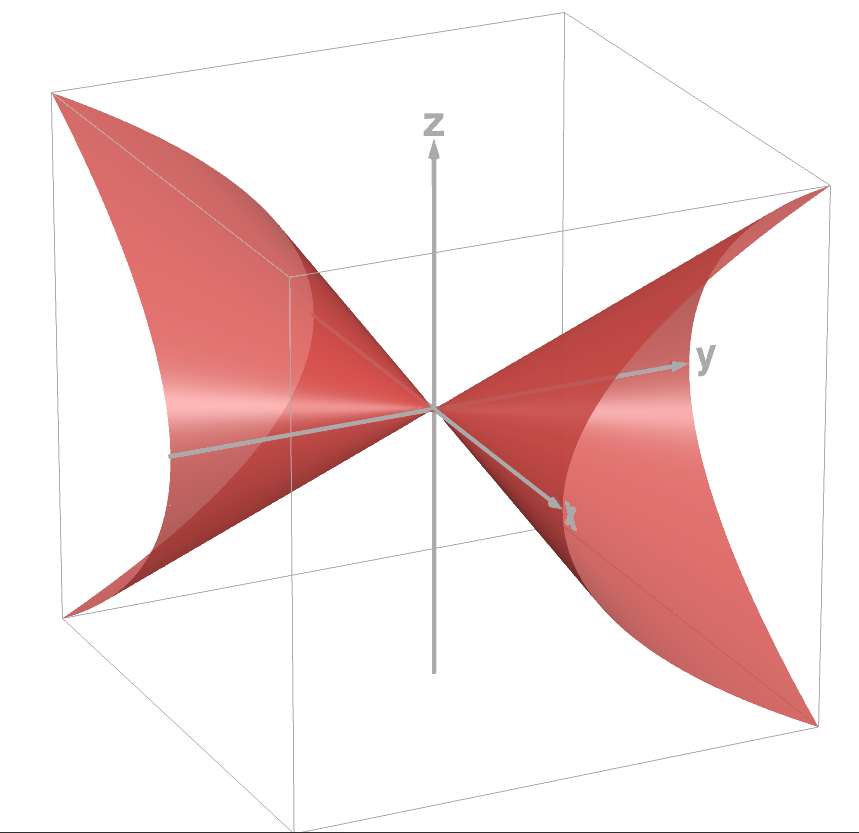
\includegraphics[width=6cm]{Images/quadric cone.png}
    \caption{Quadric cone over the real numbers.}
\end{figure}


$X$ is a toric variety with torus given by the image of\footnote{this map is 2:1, to get the actual parametrization we need
\[\funcDef{\G_m^2}{X}{(s,t)}{(s,st^2,st)}\]
This is related to the fact that $X$ is the quotient $\A^2/\mu_2$ by the action $-1(x,y)=(-x,-y)$.}
\[\funcDef{\G_m^2}{X}{(s,t)}{(s^2,t^2,st)}\]
and action
\[\funcDef{\G_m^2\times X}{X}{((s,t),(x,y,z))}{(sx,st^2y,stz)}\]
\end{example}


\begin{example}
$X=V(xy-zw)\subseteq \A^4$ is a toric variety with torus
\[\funcDef{\G_m^3}{X}{(t_1,t_2,t_3)}{(t_1,t_2,t_3,t_1t_2t_3\ii)}\]
and action 
\[\funcDef{\G_m^3\times X}{X}{((t_1,t_2,t_3),(x,y,z,w))}{(t_1x,t_2y,t_3z,t_1t_2t_3\ii w)}\]
\end{example}


\section{Monoids}

\begin{definition}[Monoid]
A \textbf{monoid} is a set $S$ with an operation $+$, which is commutative, associative and with a neutral element $0\in S$.
\end{definition}

\begin{remark}
The reference book \cite{cox2011toric} calls these \textit{semigroups}.
\end{remark}


\begin{definition}
If $A\subseteq S$ is a subset of a monoid, the \textbf{submonoid generated by $A$ in $S$} is the smallest submonoid which contains $A$. Concretely it is 
\[\ps A=\cpa{\sum_{a\in A} n_a a\mid n_a\in \N,\ n_a=0\text{ for all but finitely many coeff.}}\]
A monoid $S$ is \textbf{finitely generated} if there exists a finite subset $A\subseteq S$ such that $S=\ps A$.
\end{definition}

\begin{remark}
$S$ is a finitely generated monoid if there exists a surjective monoid homomorphism
\[\N^n\onto S.\]
\end{remark}

\begin{definition}
$S$ is an \textbf{affine monoid} if it is finitely generated and it is a submonoid of a lattice $M$.
\end{definition}

\begin{example}
$\N^k\subseteq \Z^k$ is an affine monoid.
\end{example}

\begin{example}
$\znz n$ is a monoid but it is NOT affine because a lattice can't have a submonoid with torsion.
\end{example}

\begin{example}
$\ps{(1,0),(1,1)}\subseteq \N\oplus \znz{2}$ is also not affine because of torsion.
\end{example}

\begin{definition}[Integrality]
A monoid $S$ is \textbf{integral} (or \textbf{cancellative}) if $a+b=a+c\implies b=c$.
\end{definition}

\begin{fact}
A monoid $S$ is affine if and only if $S$ is
\begin{itemize}
\item finitely generated,
\item integral and
\item torsion free.
\end{itemize}
\end{fact}

Let us now define the left adjoint to the forgetful $\Ab\to \Mon$:

\begin{definition}[Associated group]
Let $S$ be a monoid. There is an \textbf{associated abelian group} $S^{gp}$, which is the initial group with a morphism from $S$. Concretely
\[S^{gp}=\frac{\cpa{(s,s')\mid s,s'\in S}}\sim\]
where $(s_1,s'_1)\sim(s_2,s'_2)$ if there exists $s\in S$ such that\footnote{think about localization on rings which are not domains.}
\[s+s_1+s_2'=s+s_2+s_1'.\]
\end{definition}

\begin{remark}
$S^{gp}$ is an abelian group and we have a map $S\to S^{gp}$ given by $s\mapsto [(s,0)]_\sim$.
\end{remark}


\begin{fact}
Any morphism $S\to G$ for $G$ abelian group factors uniquely through $S^{gp}$. More precisely
\[\Hom_{\text{Mon}}(S,G)=\Hom_{\text{Ab}}(S^{gp},G)\]
\end{fact}


\begin{remark}
$S$ is integral if and only if $S\to S^{gp}$ is injective, which happens if and only if $S$ can be injected into an abelian group.
\end{remark}


\begin{definition}[]
A monoid is \textbf{sharp} if the only invertible element is $0$.
\end{definition}

\begin{definition}[]
An element $m$ of a sharp monoid $S$ is \textbf{irreducible} if $m=m'+m''$ in $S$ implies $m'=0$ or $m''=0$.
\end{definition}
\begin{remark}\label{ReIrreducibleGenerateForSharpMonoid}
If $S$ is a sharp monoid, the irreducible elements generate the monoid.
\end{remark}

\subsubsection{Presentations of monoids}
With monoids, the kernel is ``sort of useless"
\begin{example}
Consider
\[\funcDef{\N^2}{\N}{(a,b)}{a+b}\]
this has trivial kernel (preimage of $0$ is just $(0,0)$) but it is far from being injective.
\end{example}

Let $f:S\to S'$ be a surjective homomorphism. What we should look at instead of the kernel for the right analogue of the first isomorphism theorem is
\[E=\cpa{(s,s')\in S\times S\mid f(s)=f(s')}.\]
This set is an equivalence relation on $S\times S$, which is also a submonoid.

\begin{definition}[Congruence relations]
A submonoid of $S\times S$ which defines an equivalence relation is called \textbf{congruence relation}.
\end{definition}

\begin{definition}[Coequalizer]
If $f,g:X\to Y$, the coequalizer is an object $Z$ together with $h:Y\to Z$ such that $h\circ f=h\circ g:X\to Z$ and if $W$ together with $h':Y\to W$ is also such that $h'\circ f=c'\circ g$ then there exists a unique $Z\to W$ making everything commute.
% https://q.uiver.app/#q=WzAsNCxbMCwxLCJYIl0sWzEsMSwiWSJdLFsyLDEsIloiXSxbMiwwLCJXIl0sWzAsMSwiZiIsMCx7Im9mZnNldCI6LTF9XSxbMCwxLCJnIiwyLHsib2Zmc2V0IjoxfV0sWzEsMiwiaCIsMl0sWzEsMywiaCciXSxbMiwzLCJcXGV4aXN0cyEiLDIseyJzdHlsZSI6eyJib2R5Ijp7Im5hbWUiOiJkYXNoZWQifX19XV0=
\[\begin{tikzcd}
	&& W \\
	X & Y & Z
	\arrow["f", shift left, from=2-1, to=2-2]
	\arrow["g"', shift right, from=2-1, to=2-2]
	\arrow["{h'}", from=2-2, to=1-3]
	\arrow["h"', from=2-2, to=2-3]
	\arrow["{\exists!}"', dashed, from=2-3, to=1-3]
\end{tikzcd}\]
\end{definition}

\begin{fact}[]
We can construct quotients of $S$ by a congruence relation $E$ on $S\times S$ by setting it to be the coequalizer of $E\subseteq S\times S\rightrightarrows S$, where the arrows are the two projections from $S\times S$ to $S$.

We call this object the \textbf{quotient of $S$ by $E$} and denote it $S/E$.
\end{fact}

\begin{remark}
If $E$ is the relation constructed from $f:M\onto M'$ homomorphism of abelian groups viewed as monoids then $E=\cpa{(m,m')\in M\times M\mid f(m)=f(m')}=\cpa{(m,m')\mid m-m'\in \ker f}$. It follows that $M'\cong M/\ker f$ is a coequalizer for $E\rightrightarrows M$, so our definition makes sense.
\end{remark}


\begin{definition}[presentation of a monoid]
The monoid associated to
\[\ps{p_1,\cdots, p_r\mid a_1=b_i,\ i\in\cpa{1,\cdots, k}},\]
where $a_i,b_i,\in \ps{p_1,\cdots, p_r}_\N$, is the quotient of $\N^r$ by the congruence relation generated by the $(a_i,b_i)$ in $\N^r\times \N^r$.

A \textbf{presentation} of a monoid $S$ is an isomorphism with a monoid constructed as above.
\end{definition}





\subsection{Monoid algebra}
Since from abelian groups we costructed the group algebra and found connections to geometric objects, we want to generalize that construction to monoids.

\begin{definition}[Monoid algebra]
For a monoid $S$, its \textbf{monoid algebra} $k[S]$ is the $k$-vector space which is freely generated by $\cpa{t^s\mid s\in S}$ and with multiplication induced by the operation on $S$.
\end{definition}


\begin{remark}
In \cite{cox2011toric} they write $\chi^s$ instead of $t^s$ because they think of $S$ inside $M=X(T)$ for some torus.
\end{remark}

\begin{remark}
If $S$ is actually a group then the monoid algebra and group algebras coincide.
\end{remark}


\begin{example}
If $S=\N^n\subseteq \Z^n$ then $k[S]=k[x_1,\cdots, x_n]$.
\end{example}


\begin{proposition}
If $S$ is a monoid with presentation 
\[\ps{p_1,\cdots, p_r\mid a_i=b_i,\ 1\leq i\leq k},\] 
then
\[k[S]=\frac{k[t_1,\cdots, t_r]}{(t^{a_i}-t^{b_i})}\]
where if $a_i=\sum a_{ij}p_j$ we set $t^{a_i}=\prod t_j^{a_{ij}}$.
\end{proposition}
\begin{proof}[Sketch]
Let $R$ be the congruence relation on $\N^r$ generated by $\cpa{(a_i,b_i)}_{1\leq i\leq k}$. Since $R\rightrightarrows \N^r\to S$ is a coequalizer and $S\mapsto k[S]$ is a left adjoint ($\Hom_{\text{Mon}}(S,A)\cong \Hom_{k-\text{Alg}}(k[S],A)$) it follows that
\[k[R]\overset f{\underset g\rightrightarrows} k[\N^r]\to k[S]\] 
is a coequalizer in $k$-algebras, so $k[S]\cong k[\N^r]/I$ where $I=(f(x)-g(x)\mid x\in k[R])$.
\end{proof}



\begin{example}
Let $S=\ps{(2,0),(1,1),(0,2)}\subseteq \Z^2$. This monoid can be seen to be isomorphic to
\[\ps{p,q,r\mid p+q=2r}.\]
It follows that
\[k[S]\cong\frac{k[x,y,z]}{(xy-z^2)},\]
which is the coordinate ring of the quadric cone.
\end{example}

\begin{example}
Consider $S=\ps{2,3}\subseteq \N$, which has presentation
\[\ps{p,q\mid 3p=2q}.\]
It follows that
\[k[S]\cong \frac{k[x,y]}{(x^3-y^2)},\]
the coordinate ring of the cusp curve.
\end{example}


\section{Toric variety associated to a monoid}
Inspired by the success of Cartier duality, we consider the analogous construction with affine monoids. Instead of diagonalizable algebraic groups we will get affine toric varieties:

\begin{proposition}[]\label{PrToricVarietyAssociatedToAffineMonoid}
If $S$ is an affine monoid then
\begin{enumerate}
\item $k[S]$ is a domain and a finitely generated $k$-algebra.
\item $\Spec k[S]$ is an affine toric variety, with torus $\Spec k[S^{gp}]$.
\end{enumerate}
\end{proposition}
\begin{proof}
Let us prove the two propositions
\setlength{\leftmargini}{0cm}
\begin{enumerate}
\item Since $S\subseteq M$, we have an obvious inclusion $k[S]\subseteq k[M]$ and $k[M]$ is a domain, so $k[S]$ also is. Since $S$ is finitely generated, just take the formal variables associated to those generators and they will generate $k[S]$ as a $k$-algebra.
\item The inclusion $S\to M$ must factor through $S\to S^{gp}\to M$ by the universal property. Since $M$ is free of finite rank, $S^{gp}$ also is, thus $T=\Spec k[S^{gp}]=D(S^{gp})$ is a torus (\ref{PrCartierDualOfGeneralFinitelyGeneratedAbelianGroup}) of dimension equal to the rank of $S^{gp}$. Moreover, $k[S^{gp}]$ is a localization of $k[S]$ in a single element: if $\cpa{s_i}_{1\leq i\leq k}$ are generators of $S$ then\footnote{exercise}
\[k[S^{gp}]\cong k[S]_{\prod t^{s_i}}=k[S][t^{-s_1},\cdots,t^{-s_k}]\]
and this isomorphism is induced by the natural map $k[S]\to k[S^{gp}]$. The induced morphism $\Spec k[S^{gp}]\to \Spec k[S]$ is then an open embedding (iso. on local rings).

The translation action of $T$ on itself is the one given by
\[\funcDef{k[S^{gp}]}{k[S^{gp}]\otimes k[S^{gp}]}{t^m}{t^m\otimes t^m},\]
which extends to an action on $\Spec k[S]$ by
\[\funcDef{k[S]}{k[S^{gp}]\otimes k[S]}{t^m}{t^m\otimes t^m},\]
which makes sense because $S\subseteq S^{gp}$.
\end{enumerate}
\setlength{\leftmargini}{0.5cm}
\end{proof}

There is another construction to describe the toric variety associated to the monoid generated by a finite subset $A\subseteq M$ (recall that $M$ is the character lattice of $T$ for some torus).


Consider the morphism 
\[\phi_A:\funcDef{T_N}{(\A^1)^A}{x}{(\chi^a(x))_{a\in A}}\]
\begin{remark}
The image of $\phi_A$ is contained in the standard torus $\imm \phi_A\subseteq (\G_m)^A\subseteq (\A^1)^A$. It follows that $\imm \phi_A$ is also a torus because it is the image of a homomorphism between tori (\ref{PrImageOfTorusInATorusIsATorus}).
\end{remark}

Let $Y_A$ be the closure of $\imm \phi_A$ in $(\A^1)^A$.

\begin{proposition}[]
$Y_A$ is an affine toric variety, with torus given by the one associated to $\Z A\subseteq M$. More precisely, $Y_A\cong \Spec k[\N A]$.
\end{proposition}
\begin{proof}
The morphism $\phi_A$ corresponds to the algebra homomorphism
\[\vp_A:k[x_a\mid a\in A]\to k[M]\]
Note that 
\[\ol{\imm \phi_A}=V(\ker \vp_A)=\Spec \frac{k[x_a\mid a\in A]}{\ker\vp_A}=\Spec \imm \vp_A.\]
It is easy to see that $\imm \vp_A=k[\N A]\subseteq k[M]$. Since $\N A$ is an affine monoid we are done by (\ref{PrToricVarietyAssociatedToAffineMonoid})
\end{proof}

\begin{remark}
The two constructions are the same upon choosing a finite set of generators $A$ for $S$, letting us write $S=\N A$.
\end{remark}

\begin{definition}[Toric ideals]
The ideals of $k[\N^A]$ which give rise to toric varieties are called \textbf{Toric ideals}
\end{definition}

\begin{fact}
Toric ideals are exactly the prime ideals which can be generated by binomials (differences of monic monomials).
\end{fact}

We now want to show that this construction covers all affine toric varieties:

\begin{remark}
The torus $T_N$ acts linearly on its own ring of regular functions $k[M]$ as follows: for $t\in T_N$ and $f\in k[M]$ ($f:T_N\to \A^1$) we define\footnote{the inverse in the definition is not needed since $T_N$ is abelian, but it is put there for consistency with more general theory where it is needed to verify that the map given is indeed a left-action.} $t\cdot f\in k[M]$ as
\[t\cdot f:\funcDef{T_N}{\A^1}{p}{f({t\ii\cdot p})}\]
where the product $t\ii\cdot p$ is the product of $T_N$ as an algebraic group.

To be more precise, the action of $T_N$ is induced by a comodule structure on $k[M]$, specifically
\[k[M]\xrightarrow{\Delta}k[M]\otimes k[M]\xrightarrow{S\otimes id}k[M]\otimes k[M].\]
Technically $k[M]$ is infinite dimensional, but every time we consider this action we will actually consider the restriction to a stable finite dimensional subspace.
\end{remark}

\begin{lemma}[]\label{LmSimultaneousEigenvectorsForActionOfTorusAreTheCharacters}
The only simultaneous eigenvectors of the action $T_N\acts k[M]$ given above are the characters.
\end{lemma}
\begin{proof}
Note that $t\cdot \chi^m (p)=\chi^m(t\ii\cdot p)=\chi^m(t\ii)\chi^m(p)$ on the torus, thus $t\cdot \chi^m=\chi^m(t\ii) \chi^m$, that is, characters are simultaneous eigenvectors for this action of $T_N$. 

Let us now prove that they are the only ones (up to scalars):
if $\sum a_m \chi^m$ in $k[M]$ is a simultaneous eigenvector then 
\[\al(t)\pa{\sum a_m \chi^m}=t\cdot \pa{\sum a_m \chi^m}=\sum \chi^m(t\ii)a_m \chi^m\]
for some function $\al:T_N\to k$, thus $a_m\al(t)=a_m\chi^m(t\ii)$ for all $m$. If $a_{m_1}\neq 0\neq a_{m_2}$ then $\chi^{m_1}(t\ii)=\al(t)=\chi^{m_2}(t\ii)$, so $m_1=m_2$ and thus the simultaneous eigenvector we chose must be of the form $a_m \chi^m$ for some $m\in M$.
\end{proof}

\begin{lemma}
If $A\subseteq k[M]$ is a subspace which is stable under the action above then
\[A=\bigoplus_{t^m\in A}k t^m,\]
that is, $A$ is generated by characters.
\end{lemma}
\begin{proof}
Call $A'=\bigoplus_{t^m\in A}k t^m$. Clearly $A'\subseteq A$ so we just need the other inclusion. Pick $f\in A$ and write
\[f=\sum_{m\in B}c_m t^m\]
for $B\subseteq M$ finite and such that $c_m\neq 0$ for all $m\in B$. Note that
\[f\in A\cap \ps{t^m\mid m\in B}:=V.\]
This intersection is a finite dimensional $k$-vector space which is stable under the $T_N$-action, so it is a finite dimensional representation of $T_N$. By proposition (\ref{PrRepresentationsOfToriSplit}) it follows that $V$ is generated by simultaneous eigenvectors of the action, which are the $t^m$ by the lemma above. Writing what we have just said in symbols: 
\[f\in V=\bigoplus_{\smat{m\in B\ s.t.\\ t^m\in A}}kt^m\subseteq \bigoplus_{t^m\in A}k t^m=A'.\]
\end{proof}

\begin{theorem}[]\label{ThAffineToricVarietiesComeFromAffineMonoids}
All affine $T_N$-toric varieties are isomorphic to one of the form $\Spec k[S]$ for some monoid $S\subseteq M=X(T_N)$.
\end{theorem}
\begin{proof}
If $X=\Spec A$ is an affine toric variety, then $A\subseteq k[M]$ is stable for the action of $T_N$ on $k[M]$. This is because $\cdot t\ii:T_N\to T_N$ extends to $X$ by definition of toric variety.
By the lemma above
\[A=\bigoplus_{t^m\in A}k t^m=k[S],\]
where $S=\cpa{m\in M\mid t^m\in A}$, which is a submonoid of $M$ because $A$ is an algebra.

Since $A$ is finitely generated, there exist $f_1,\cdots, f_k$ such that $A=k[f_1,\cdots, f_k]$. By replacing each $f_i$ with all the characters that you need to write it out, we can assume that the $f_i$ are all of the form $t^m$.

It is now easy to check that the corresponding exponents generate $S$.
\end{proof}



\section{Cones}
It will turn out that (normal) affine toric varieties are described by cones lying in $N_\R=N\otimes_\Z\R$ where $N$ is a lattice (it will be the cocharacter lattice of the resulting toric variety).

\begin{definition}[]
A \textbf{convex polyhedral cone} (from now on just \textbf{cone}) is a subset of $N_\R$ of the form
\[\sigma=\Cone(A)=\cpa{\sum_{n\in A}\la_n\cdot n\mid \la_n\geq 0}\subseteq N_\R\]
where $A\subseteq N_\R$ is a finite subset.
\end{definition}

\begin{remark}
A cone $\sigma$ is a convex subset of $N_\R$ and it is a ``positive" cone, in the sense that if $v\in \sigma$ and $\la\in [0,+\infty)\subseteq \R$ then $\la v\in \sigma$.
\end{remark}

\begin{example}
The positive quadrant 
\[\cpa{(x,y)\in \R^2\mid x\geq 0,\ y\geq 0}=\Cone((1,0),(0,1))\] 
is a cone.
$\Cone((1,0),(1,2))$ is also a cone, which is embedded differently.
\end{example}

\begin{definition}[Orthant]
An \textbf{orthant} is a cone of the form $\Cone(e_1,\cdots, e_k)\subseteq \R^n$.
\end{definition}

\begin{example}
$\Cone((1,0,0),(0,1,0),(1,0,1),(0,1,1))\subseteq \R^3$ is a cone.
\end{example}

\begin{example}
A line in $\R^2$ is a cone, since it can be written $\Cone(v,-v)$. In general linear subspaces are cones.
\end{example}


\begin{definition}[]
A cone $\sigma$ is \textbf{strongly} or \textbf{strictly convex} if it does not contain any positive dimensional subspace.
\end{definition}

\begin{definition}[]
The \textbf{dimension} of $\sigma$, denoted $\dim\sigma$, is the dimension of the vector subspace of $N_\R$ spanned by $\sigma$.

A cone is \textbf{full-dimensional} if its dimension is the same as the rank of $N$.
\end{definition}


\subsection{General facts about cones}
For references you can look at Fulton \cite{fulton1993introduction} for most of these facts.

\begin{proposition}
A cone is closed in the respective $N_\R$.
\end{proposition}
\begin{proof}[Sketch]
Assume the following theorem by Carath\'eodory: \textit{if $v\in \Cone(A)$ then there exists $B\subseteq A$ linearly independent such that $v\in \Cone(B)$.}
\medskip

\noindent
It follows that
\[\Cone(A)=\bigcup_{\smat{B\subseteq A\\B\text{ lin. ind.}}}\Cone(B)\]
and this is a finite union of closed sets because $\Cone(B)$ can be identified with $\R^{k}_{\geq 0}\times \R^{n-k}$ via a linear transformation for some $k$.
\end{proof}

\begin{definition}[]
Two polytopes are said to be \textbf{combinatorially equivalent} if their poset of faces are isomorphic.
\end{definition}

Is there any polytope which is combinatorially equivalent to one with rational vertices (i.e. vetices in $\Q^n$)? Surprisingly, no. In all dimensions above 8 there are some polytopes that contradict this (which is weird because one would think ``I can just move the vertices a little").

For more details look up \textit{non-realizable matroids}.

\subsubsection{Hyperplanes and dual cone}
\begin{definition}[Hyperplane and closed half-space]
If $m\in M_\R$, we write
\[H_m=\cpa{n\in N_\R\mid \ps{m,n}=0}\]
(the product is the one induced by $M\times N\to \Z$ upon tensoring with $\R$). Sets of this form are \textbf{hyperplanes} in $N_\R$.

We write $H_m^+$ for $\cpa{n\in N_\R\mid \ps{m,n}\geq 0}$ and call this a \textbf{closed half-space}.
\end{definition}

\begin{definition}[]
$H_m$ is a \textbf{supporting hyperplane} for a cone $\sigma$ if $\sigma\subseteq H_m^+$. We call $H_m^+$ a \textbf{supporting half-space}.
\end{definition}


\begin{definition}[]
The \textbf{dual cone} to a cone $\sigma$ is
\[\sigma^\vee=\cpa{m\in M_\R\mid \ps{m,n}\geq 0\ \forall n\in \sigma}\subseteq M_\R\]
\end{definition}

\begin{remark}
By definition 
\[\sigma^\vee=\bigcap_{\smat{m\in M_\R\ s.t.\\ H_m^+\text{ supp. half-sp.}}}H_m^+,\] so $H_m$ is supporting if and only if $m\in \sigma^\vee\nz$.
\end{remark}

\begin{fact}
$\sigma^\vee$ is also a cone and $(\sigma^\vee)^\vee\cong \sigma$ under the identification $(N_\R^\vee)^\vee\cong N_\R$.
\end{fact}

\begin{fact}
$m_1,\cdots, m_s$ generate $\sigma^\vee$ if and only if $\sigma=H_{m_1}^+\cap\cdots\cap H_{m_s}^+$.
In particular, every cone is a finite intersection of half-spaces.
\end{fact}

\begin{definition}[]
A \textbf{face} of a cone $\sigma$ is a subset of the form $\tau=\sigma\cap H_m$ for some $m\in \sigma^\vee$. In this case we write $\tau\leq \sigma$.
\end{definition}
\begin{figure}[!htb]
	\centering
	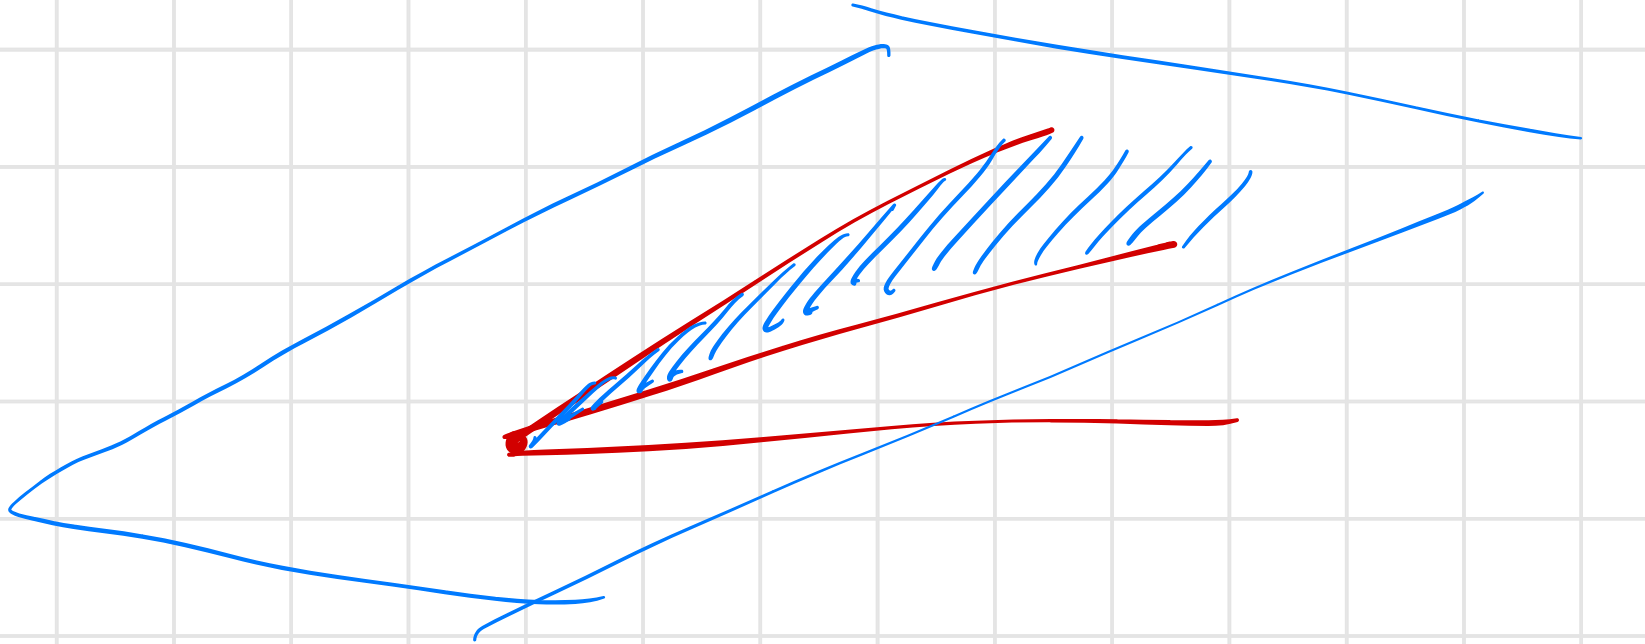
\includegraphics[width=7cm]{Images/face.png}
\end{figure}



\begin{remark}
If $\sigma=\Cone(A)$ then $\tau=\Cone(a\in A\mid a\in H_m)$. In particular $\tau$ is also a cone.
\end{remark}


\begin{definition}[]
A face is \textbf{proper} if it is not $\sigma$ itself.
\end{definition}

\begin{fact}
The following are true:
\begin{itemize}
\item If $\tau_1,\tau_2\leq \sigma$ then $\tau_1\cap \tau_2\leq \sigma$
\item if $\tau'\leq \tau$ and $\tau\leq \sigma$ then $\tau'\leq \sigma$
\item if $\tau\leq \sigma$ and $v,w\in \sigma$ are such that $v+w\in \tau$ then $v,w\in \tau$.
\end{itemize}
\end{fact}



\begin{definition}[]
A \textbf{ray} (or \textbf{edge}) is a 1 dimensional face. A \textbf{facet} is a $\dim\sigma-1$ dimensional face.
\end{definition}


\begin{fact}
If $\sigma$ is full-dimensional in $N_\R$ then in the representations like $\sigma=H_{m_1}^+\cap\cdots\cap H_{m_s}^+$ we can assume that $\sigma\cap H_{m_i}$ is a facet of $\sigma$ for all $i$.
\end{fact}

\begin{remark}
This is not the case if $\sigma$ is not full-dimensional, for example for $\sigma=\Cone((1,0))\subseteq \R^2$ the only facet is $\cpa{(0,0)}$ but in order to write $\sigma$ as the intersection of half-spaces we need some half-spaces with associated hyperplane being $\Span((1,0))$ and so $\sigma\cap H$ for those hyperplanes is $\sigma$ itself.
\end{remark}


\begin{fact}
Every proper face is the intersection of all facets containing it.
\end{fact}


\begin{remark}
If $N_\R\cong \R^n$ then we know that $M_\R\cong \R^n$ via the dual basis and we can think of one of the $m_i$ that generate the dual cone as an ``inward-pointing" normal vector to a facet of $\sigma$
\end{remark}


\begin{example}
Let $\sigma=\Cone((1,0),(1,2))$. 
\begin{figure}[!htb]
	\centering
	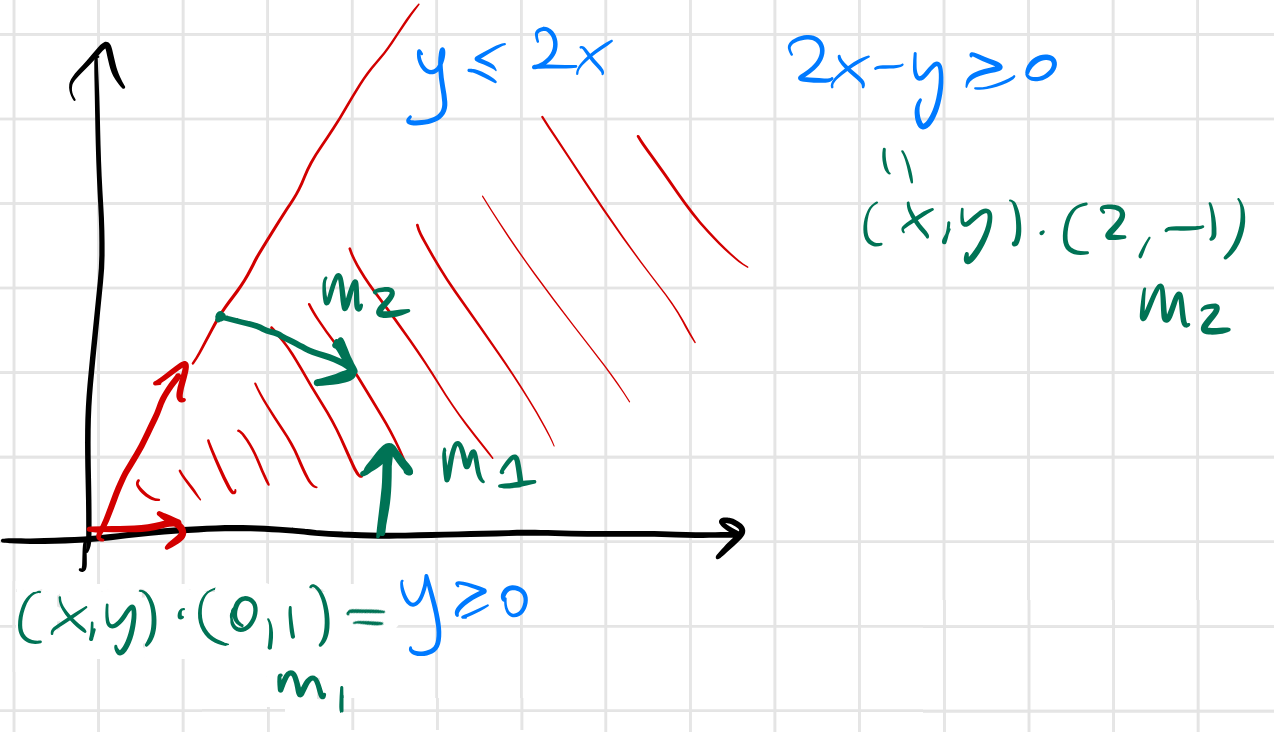
\includegraphics[width=7cm]{Images/Inward-facing-normals-for-dual-cone.png}
\end{figure}

\noindent
The half-planes that bound the cone are $y\geq 0$ and $2x-y\geq0$, which correspond to $(0,1)$ and $(2,-1)$, which can be used to generate $\sigma^\vee=\Cone((0,1),(-2,1))$.
\end{example}


\begin{example}
Take $\sigma=\Cone((1,0))\subseteq \R^2$, so $\sigma^\vee$ is $\Cone((1,0),(0,1),(0,-1))$ which correspond to $x\geq 0$, $y\geq 0$ and $-y\geq 0$
\end{example}

\begin{fact}
The following are equivalent:
\begin{itemize}
\item $\sigma$ is strictly convex,
\item $\cpa{0}$ is a face of $\sigma$,
\item $\sigma\cap (-\sigma)=\cpa{0}$,
\item $\dim \sigma^\vee=\dim M_\R$.
\end{itemize}
\end{fact}

\begin{fact}
Any cone $\sigma$ contains a maximal linear subspace given by $\sigma\cap (-\sigma)=W$. Moreover, $\sigma/W\subseteq N_\R/W$ is strictly convex.
\end{fact}


\begin{definition}[]
$\sigma$ is \textbf{rational} if $\sigma=\Cone(A)$ for $A\subseteq N$ (not $N_\R$ like before).
\end{definition}



\begin{fact}
	The dual and the faces of a rational cone are rational.
\end{fact}

\begin{fact}
If $A\subseteq N$ then 
\[\Cone(A)\cap N_\Q=\cpa{\sum_{a\in A} q_a a\mid q_a\in \Q}.\]
\end{fact}

\begin{definition}[]
Let $\sigma$ be a rational cone, its \textbf{minimal ray generators} are given as follows: if $\rho\leq \sigma$ is a ray (and thus rational), the minimal ray generator correspondint to it is the minimal generator of $\rho\cap N$ as a monoid, which is denoted $u_\rho$.
\end{definition}

\begin{fact}
A strictly convex rational cone is ``canonically" generated by its minimal ray generators:
\[\sigma=\Cone(u_\rho\mid \rho\text{ is a ray}).\]
\end{fact}

\begin{corollary}
If $\sigma$ is a rational full-dimensional cone then $\sigma$ has minimal facet normals (minimal ray generators of the dual).
\end{corollary}




\section{Affine toric varieties from cones}

\begin{notation}
Let $\sigma$ be a cone in $N_\R$. We write
\[S_\sigma=\sigma^\vee\cap M.\]
\end{notation}
\begin{remark}
$S_\sigma$ is a submonoid of $M$ because if $m,m'\in \sigma^\vee\cap M$ then
\[\ps{m+m',n}=\ps{m,n}+\ps{m'n}\geq 0+0=0.\]
\end{remark}

\begin{lemma}[Gordan]\label{LmGordan}
If $\sigma$ is a rational polyhedral cone in $N_\R$, then $S_\sigma=\sigma^\vee\cap M$ is finitely generated. 
\end{lemma}
\begin{proof}
Write $\sigma^\vee=\Cone(T)$ with $T\subseteq M$ some finite subset. Consider
\[K=\cpa{\sum_{m\in T}a_m m\mid 0\leq a_m<1}.\]
Clearly $K$ is bounded in $M_\R$, so $K\cap M$ is a finite set. We claim that $T\cup (K\cap M)$ generates $S_\sigma$ as a monoid:

Let $w\in S_\sigma=\sigma^\vee\cap M$. We can write $w=\sum_{m\in T}\la_m m$ with $\la_m>0$ real numbers. We can write $\la_m=\floor{\la_m}+\cpa{\la_m}$ (floor and fractional part), so that
\[w=\under{\in M}{\sum_{m\in T}\floor{\la_m}m}+\under{\in K}{\sum_{m\in T}\cpa{\la_m}m}.\]
But $\sum_{m\in T}\cpa{\la_m}m$ is also in $M$ because it is $w- \sum_{m\in T}\floor{\la_m}m$, so we have written $w$ in the desired form.
\end{proof}

Because of the correspondence between affine toric varieties and affine monoids that we built (\ref{PrToricVarietyAssociatedToAffineMonoid}) we can give the following definition:

\begin{definition}[]
Let $\sigma\subseteq N_\R$ be a rational cone. Its affine toric variety is
\[U_\sigma=\Spec k[S_\sigma].\]
\end{definition}


\begin{remark}
The torus of $U_\sigma$ has character lattice $S_\sigma^{gp}\subseteq M$.
\end{remark}

\begin{remark}
Why are we not taking $\Spec[\sigma\cap M]$ (for $\sigma$ cone in $M_\R$) instead? This is because the gluing process of affine pieces will be more natural if the cones are in $N_\R$
\end{remark}

\begin{proposition}
The following are equivalent
\begin{enumerate}
\item $\dim U_\sigma=n=\dim N_\R$
\item the torus of $U_\sigma$ is $T_N$
\item $\sigma$ is strictly convex.
\end{enumerate}
\end{proposition}
\begin{proof}
First note that 
\[\dim U_\sigma=\rnk S^{gp}_\sigma=\dim \Cone(S_\sigma)=\dim\sigma^\vee\]
From this, $\dim U_\sigma=n$ is equivalent to $\dim \sigma^\vee=n$ which we know is equivalent to $\sigma$ being strongly convex.

For the other equivalence, we claim $M/S^{gp}_\sigma$ is torsion free. This gives the desired equivalence because we get
\[\dim U_\sigma=n\coimplies\rnk S^{gp}_\sigma=\rnk M\overset{\text{claim}}\coimplies M=S_\sigma^{gp}\coimplies T_N\text{ is the torus in }U_\sigma.\] 
We now prove that the claim holds. Let $m\in M$ and assume that $km\in S^{gp}_\sigma$ for some $k\in \N$. Then $km=m_1-m_2$ for some $m_1,m_2\in S_\sigma$ and so
\[M\ni m+m_2=\frac1k m_1+\frac{k-1}km_2\in \sigma^\vee\]
where the last inclusion holds by convexity. Thus $m=(m+m_2)-m_2$ implies $m\in S^{gp}_\sigma$
\end{proof}

\begin{center}
	Because of this result, from now on a cone $\sigma$ will be assumed to be strictly convex (i.e. $S_\sigma^{gp}=M$) and rational unless otherwise stated.
\end{center}




\begin{example}
Let $\sigma=\Cone(e_1)\subseteq \R^2$, then $\sigma^\vee=\Cone(e_1,e_2,-e_2)$
\end{example}

\begin{example}
If $\sigma=\Cone(e_1,\cdots, e_k)\subseteq \R^n$ is an orthant then 
\[\sigma^\vee=\Cone(e_1,\cdots, e_k, \pm e_{k+1},\cdots, \pm e_n).\]

It follows that $k[S_\sigma]=k[x_1,\cdots, x_k,x_{k+1}^{\pm1},\cdots,x_n^{\pm1}]$ and so for an orthant
\[U_\sigma\cong \A^k\times \G_m^{n-k}.\]
\end{example}

\begin{example}
If $\sigma=\Cone(0)=\cpa{0}$ then $\sigma^\vee=M$ and so $U_\sigma=T_N$
\end{example}

\begin{example}[Rational normal cone of degree $d$]
Let $d\in \N\nz$ and take $\sigma=\Cone(de_1-e_2,e_2)$

\begin{figure}[!htb]
	\centering
	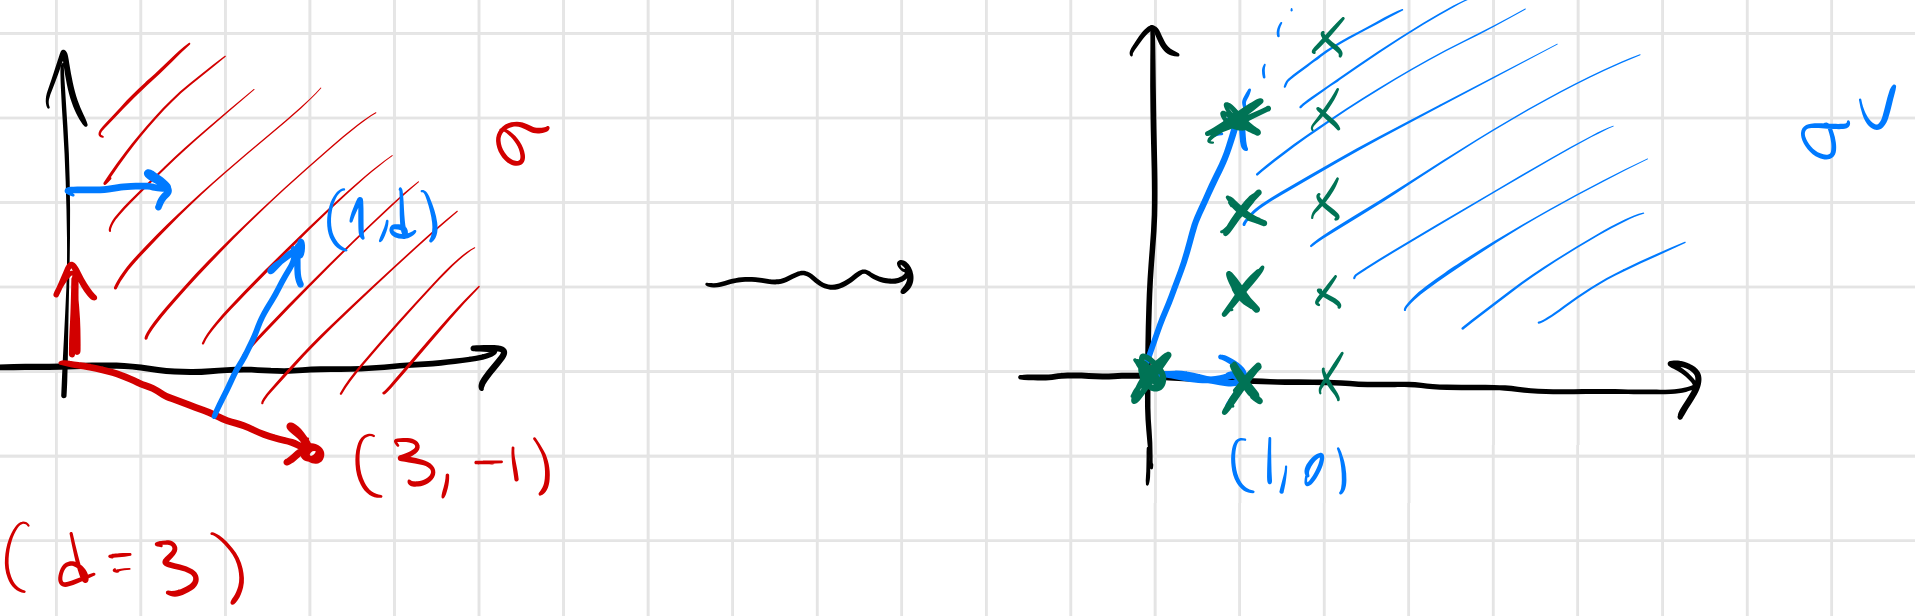
\includegraphics[width=9cm]{Images/Rational-normal-cone-cone.png}
\end{figure}

\noindent
It turns out that $S_\sigma=\ps{(1,i)\mid 0\leq i\leq d}$ (not trivial yet). Let us study
\[U_\sigma=\Spec k[S_\sigma]\]
Setting $A=\cpa{(1,i)\mid 0\leq i\leq d}$, we can see $U_\sigma$ as $Y_A$, the closure of the image of
\[\funcDef{\G_m^2}{\A^{d+1}}{(s,t)}{(s,st^1,\cdots, st^d)}\]
\end{example}

\begin{definition}
The toric variety from the previous example is called the \textbf{rational normal cone of degree $d$}. It is the affine cone over the so called \textit{rational curve of degree $d$} in $\Pj^d$.
\end{definition}

\begin{remark}
It turns out that the ideal of the rational normal cone of degree $d$ is $(x_ix_{j+1}-x_{i+1}x_j\mid 0\leq i<j\leq d)$. Note that the generators are determinants of $2\times 2$ matricies, specifically, all minors of
\[\mat{x_0 & \cdots & x_{d-1}\\ x_1 & \cdots & x_d}\]
\end{remark}

\begin{example}
Consider $\sigma=\Cone(e_1,e_2,e_1+e_3,e_2+e_3)$. The equations that define this cone are $y\geq 0$, $z\geq 0$, $x\geq 0$ and $x+y-z\geq 0$, so $\sigma^\vee=\Cone(e_1,e_2,e_3,e_1+e_2-e_3)$.

You can check that $S_\sigma=\sigma^\vee\cap M\cong\ps{p,q,r,s\mid p+q=r+s}$, showing that
\[k[S_\sigma]\cong \frac{k[x,y,z,w]}{(xy-zw)}.\]
\end{example}

\begin{remark}
When $\sigma$ is full-dimensional ($\sigma^\vee$ is strictly convex) it follows that $S_\sigma$ is sharp and so (\ref{ReIrreducibleGenerateForSharpMonoid}) the irreducible elements of $S_\sigma$ give a canonical generating set.
\end{remark}

\begin{definition}[]
Let $\sigma$ be a cone. If $S_\sigma$ is sharp, the set 
\[H=\cpa{m\in S_\sigma\mid m\text{ irreducible}}\]
is called the \textbf{Hilbert basis} of $S_\sigma$.
\end{definition}


\begin{fact}
If $\sigma$ is full dimensional (and so $S_\sigma$ is sharp) then
\begin{itemize}
\item $H$ is finite and generates $S_\sigma$
	\item $H$ contains the minimal generators of the rays of $\sigma^\vee$
	\item every generating set of $S_\sigma$ contains $H$
\end{itemize}
\end{fact}


\section{Normality and smoothness of affine toric varieties}
\subsection{Normality}
\begin{definition}[]
If $X=\Spec A$ is an irreducible affine algebraic variety ($A$ is a domain) then $X$ is \textbf{normal} if $A\subseteq \Frac A$ is integrally closed.
\end{definition}

\begin{remark}
$X$ is normal if and only if all local rings of $X$ are integrally closed in $\Frac A$. We are identifying the local rings with the subrings of $\Frac A$ below
\[A_{\mf_p}\cong \Oc_{X,p}=\cpa{f\in \Frac A\mid f=\frac gh,\ h(p)\neq 0}.\]
\end{remark}

\begin{definition}[]
An integral monoid $S$ is \textbf{saturated} if for all $s\in S^{gp}$ such that there exists $k\in \N\nz$ such that $ks\in S$ we have $s\in S$.
\end{definition}

\begin{example}
$S=\ps{2,3}\subseteq \N$ is not saturated because $S^{gp}=\Z$ ($1=3-2$) and $2\cdot 1=2\in S$ but $1\notin S$.
\end{example}

\begin{remark}
In \cite{cox2011toric} they say that $S\subseteq M$ is saturated if the condition holds for $m\in M$. The two definitions are not equivalent because $2\N\subseteq\Z$ is saturated for our definition but not theirs.

If $S^{gp}=M$ the two definitions are the same and this is always assumed in \cite{cox2011toric} so nothing really changes but the true definition in monoid theory is the one we gave.
\end{remark}

\begin{proposition}[]\label{PrCriteriaForNormalAffineToricVariety}
For an affine toric variety $X$ with torus $T_N$, the following are equivalent
\begin{enumerate}
\item $X$ is normal
\item $X=\Spec k[S]$ for $S$ saturated
\item There exists a strictly convex cone $\sigma$ in $N_\R$ with $X\cong U_{\sigma}$
\end{enumerate}
\end{proposition}
\begin{proof}
Let us give the implications
\setlength{\leftmargini}{0cm}
\begin{itemize}
\item[$\boxed{1\implies2}$] Suppose $X$ is normal and let $S\subseteq M$ be some monoid such that $S^{gp}=M$ and $X\cong \Spec k[S]$. Let $m\in S^{gp}=M$ and $k\in\N\nz$ be such that $km\in S$, then $t^{km}\in k[S]$ and $t^m\in k[M]\subseteq \Frac(k[S])$ is a root of the polynomial
\[y^k-t^{km}\in k[S][y].\]
Since $k[S]$ is integrally closed we get $t^m\in k[S]$ and so $m\in S$
\item[$\boxed{2\implies3}$] Suppose $S$ is saturated with $S^{gp}=M$. Let $A\subseteq S$ be a set of generators and take $\tau=\Cone(A)\subseteq M_\R$. Define $\sigma=\tau^\vee$. This $\sigma$ is strictly convex because $\tau$ is full dimensional by construction and clearly $S\subseteq \tau\cap M=\sigma^\vee\cap M$. We just need the other inclusion now. If $m\in \tau\cap M$ then $m\in M\subseteq M_\Q$ and so
\[m=\sum_{a\in A}q_a a\]
for some $q_a\in \Q$, $q_a\geq 0$. Upon taking the least common multiple of the denominators $N$ we get a positive integer such that $Nm$ is an integral linear combination of the elements of $A$, thus $Nm\in S$ and by saturatedness we have $m\in S$ as desired.
\item[$\boxed{3\implies1}$] Let $\rho_1,\cdots, \rho_r$ be the rays of $\sigma$, then $\sigma^\vee=\bigcap_{i=1}^r\rho_i^\vee$ and so
\[k[S_\sigma]=\bigcap_{i=1}^r k[S_{\rho_i}]\subseteq k[M].\]
Since the intersection of integrally closed subrings is integrally closed we may suppose without loss of generality that $\sigma=\rho$ is a ray. 

Let $u_\rho$ be the minimal ray generator of $\rho$, then we can complete $u_\rho$ to a $\Z$-basis of $N$: consider the exact sequence ($N'=\coker(\ps{u_\rho}\subseteq N)$)
\[0\to \ps{u_\rho}\to N\to N'\to 0\]
Note that $N'$ is torsion free and thus free (finitely generated abelian group), so the sequence splits and we have $N\cong \ps{u_\rho}\oplus N'$.

We may therefore assume that $\rho=\Cone(e_1)$, so that $\rho^\vee=\Cone(e_1,\pm e_2,\cdots, \pm e_n)$, so $k[S_\rho]=k[x_1,x_2^{\pm 1},\cdots, x_n^{\pm 1}]$ and this is integrally closed.
\end{itemize}
\setlength{\leftmargini}{0.5cm}
\end{proof}



\begin{remark}
If $S$ is integral but not saturated then it has a saturation $S^{sat}$ given by $\cpa{m\in S^{gp}\mid \exists k>0,\ km\in S}$. Note that 
\begin{itemize}
\item $S\subseteq S^{sat}\subseteq S^{gp}$
\item $S^{sat}$ is finitely generated
\item $(S^{sat})^{gp}=S^{gp}$
\end{itemize}
Moreover, the inclusion $k[S]\to k[S^{sat}]$ gives the ``normalization" $\Spec k[S^{sat}]\to \Spec k[S]$
\end{remark}

\begin{example}
Let $S=\ps{2,3}\subseteq \N$ and note that $S^{sat}=\N$. Recall that $\ps{2,3}=\ps{p,q\mid 3p=2q}$, so
\[k[S]=\frac{k[x,y]}{(x^3-y^2)}\]
and $C=\Spec k[S]$ is the cuspidal cubic in $\A^2$ (not normal variety). The normalizaion of this is
\[\funcDef{\A^1}{C\subseteq \A^2}{t}{(t^2,t^3)}\]
\end{example}


\begin{example}
Consider the monoid $S=\ps{(2,0),(1,1),(0,2)}\subseteq \Z^2$. We know that $\Spec k[S]$ is a normal variety, but the monoid does not ``look" saturated. For example, $(0,1)\in \Z^2\bs S$ but $2(0,1)=(0,2)\in S$. The issue is that $S^{gp}$ is smaller than $\Z^2$ and $(0,1)\notin S^{gp}$.
\end{example}

\subsection{Smoothness}

\begin{remark}
Recall that $T_xX=({\mf_x}/{\mf_x^2})^\vee$ in general. If $X\subseteq \A^n$ as $V(I)$ with $I=(f_1,\cdots, f_s)$ then $T_xX$ is defined by the linear equations $0=d_x(f_i)=\sum_{j=1}^n \pp{x_j}{f_i}(x)x_j$ with $1\leq i\leq n$.
\end{remark}

\begin{definition}[]
An irreducible affine variety $X=\Spec A$ is \textbf{smooth} if $\dim T_xX=\dim X$ for all $x\in X$.
\end{definition}

\begin{fact}[Jacobian criterion]
An irreducible $X=V(f_1,\cdots, f_s)\subseteq \A^n$ of dimension $d$ is smooth at $x\in X$ if and only if
\[\rnk\mat{\displaystyle\pp{x_j}{f_i}(x)}=n-d.\]
\end{fact}

\noindent
We will see that an affine toric variety $U_\sigma$ is smooth if and only if $\sigma$ is a \textit{smooth cone}:

\begin{definition}[]
A rational strongly convex cone $\sigma\subseteq N_\R$ is
\begin{itemize}
\item \textbf{smooth} (or \textbf{regular}) if the minimal ray generators of $\sigma$ are part of a $\Z$-basis of $N$
\item \textbf{simplicial} if the minimal ray generators are $\R$-linearly independent in $N_\R$.
\end{itemize}
\end{definition}

\begin{example}
The cone $\R_{\geq0}^k\subseteq \R^n$ is smooth. Moreover, all smooth cones are of this form up to the action of some element of $\GL(\Z,n)$.
\end{example}

\begin{example}
The cone $\sigma=\Cone((1,0),(1,2))$ is simplicial because $(1,0)$ and $(1,2)$ are linearly independent, but $(1,0)$ and $(1,2)$ cannot be part of a basis for $\sigma$ because the element $(1,1)$ would never be reached despite being in the cone.
\end{example}

\begin{example}
The cone $\Cone((1,0,0), (0,1,0), (1,0,1),(0,1,1))\subseteq \R^4$ is not simplicial because it has 4 minimal ray generators.
\end{example}

\begin{remark}
Points of $\Spec k[S]$ are in bijection with homomorphisms of monoids $S\to (k,\cdot)$:
\begin{align*}
	\cpa{\text{points of }\Spec k[S]}\overset{NSS}=&\cpa{\text{max. ideals of }k[S]}=\\
	=&\cpa{\text{surjections of $k$-algebras }k[S]\to k}=\\
	=&\cpa{\text{monoid homomorphisms }S\to (k,\cdot)}
\end{align*}
where the last equality works because it amounts to choosing a value in $k$ for each $s\in S$ (or equivalently $t^s\in k[S]$) which is compatible with the operations. The surjectivity works because $S\to (k,\cdot)$ being a homomorphism means that $0$ goes to $1$ and so the corresponding $k$-alegbra homomorphism has $1$ in the image, making the map surjective.
\end{remark}

\begin{lemma}[]\label{LmFixedPointForActionOfTorusInAffine}
The action of $T_N$ on $\Spec k[S]$ has a fixed point if and only if $S$ is sharp.
In this case there is exactly one fixed point, which corresponds to $S\to (k,\cdot)$ given by $s\mapsto \begin{cases}
	0&\text{if }s\neq 0\\
	1&\text{if }s=0
\end{cases}$
\end{lemma}
\begin{proof}
If $p\in \Spec k[S]$ corresponds to $\gamma:S\to (k,\cdot)$ and we fix $a\in T_N$, let us compute $a\cdot p$: recall that the action is described by
\[\funcDef{k[S]}{k[M]\otimes k[S]}{t^s}{t^s\otimes t^s}\]
and so it maps $(a,p)\in T_N\times X$ to the point which corresponds to $k[S]\to k$ given by
% https://q.uiver.app/#q=WzAsNixbMCwwLCJrW1NdIl0sWzEsMCwia1tNXVxcb3RpbWVzIGtbU10iXSxbMiwwLCJrXFxvdGltZXMgaz1rIl0sWzAsMSwidF5zIl0sWzEsMSwidF5zXFxvdGltZXMgdF5zIl0sWzIsMSwiXFxjaGlecyhhKVxcZ2FtbWEocykiXSxbMCwxXSxbMSwyXSxbMyw0LCIiLDAseyJzdHlsZSI6eyJ0YWlsIjp7Im5hbWUiOiJtYXBzIHRvIn19fV0sWzQsNSwiIiwwLHsic3R5bGUiOnsidGFpbCI6eyJuYW1lIjoibWFwcyB0byJ9fX1dXQ==
\[\begin{tikzcd}
	{k[S]} & {k[M]\otimes k[S]} & {k\otimes k=k} \\
	{t^s} & {t^s\otimes t^s} & {\chi^s(a)\gamma(s)}
	\arrow[from=1-1, to=1-2]
	\arrow[from=1-2, to=1-3]
	\arrow[maps to, from=2-1, to=2-2]
	\arrow[maps to, from=2-2, to=2-3]
\end{tikzcd}\]
so the homomorphism $\gamma':S\to (k,\cdot)$ which corresponds to $a\cdot p$ is given by $\gamma'(s)=\chi^s(a)\gamma(s)$.

The point is fixed if $\chi^s(a)\gamma(s)=\gamma(s)$ for all $a\in T_N,\ \in S$. For $s= 0$ $\gamma(s)=1$ ok because it has to be a homomorphism, for $s\neq 0$ this implies that $\gamma(s)=0$ in $k$ (because $\exists a\in T_N$ such that $\chi^s(a)\neq 1$), so the only possible $\gamma$ is the one in the statement, which is a homomorphism if and only if $S$ is sharp.
\end{proof}

\begin{remark}
The point in the statement of the lemma above can be thought of as the ``most singular point of $X$".
\end{remark}	










